%%%%%%%%%%%%%%%%%%%%%%%%%%%%%%%%%%%%%%%%%%%%%%%%%%%%%%%%%%%%%%%%%%%%%
%                                                                   %
%	CHAPTER ONE, MODELS of HPC                                       %
%                                                                   %
%%%%%%%%%%%%%%%%%%%%%%%%%%%%%%%%%%%%%%%%%%%%%%%%%%%%%%%%%%%%%%%%%%%%%

\chapter{Models for HPC}

\section{Introduction}

High Performance Computing (HPC) takes its roots from the beginning of computer odyssey in the middle of 20th century.
A lot of rules, observations and theories emerged from it and most of the Computer Science fields. 
In order to understand and characterize HPC and supercomputers, some knowledge on theory is required. 
This part describes the Von Neumann model, the generic model of sequential computer on which every nowadays machine is built.
It is presented along with the Flynn taxonomy that is a classification of the different execution models. 
We also present the different memory models based on those elements. 

Then we give more details on what parallelism is and how to reach performances though it. 
And thus we define what performance implies in HPC. 
The Amdahl's and Gustafson's laws are presented and detailed along with the strong and weak scaling used in our study. 

\section{Von Neumann Model}
\index{Von Neumann Model}
First computers, in early 20th century, were built using vacuum tubes making them high power consuming, hard to maintain and expensive to build.
The most famous of first vacuum tubes supercomputers, the ENIAC, was based on a decimal system.
It might be the most known of first supercomputers but the real revolution came from its successor.
In 1944 the first binary system based computer was created, called the Electric Discrete Variable Automatic Computer (EDVAC). 
In the EDVAC team, a physicist described the logical model of this computer and provided a model on which every nowadays computing device is based. 

\begin{figure}
\centering 
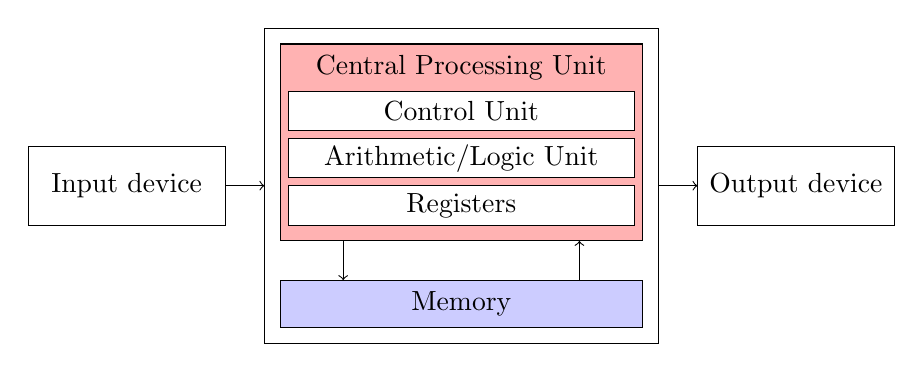
\begin{tikzpicture}
\draw (3,0) rectangle (8,4);
\draw (3.2,1.3) [fill=red!30] rectangle (7.8,3.8);
\node at (5.5,3.5) {Central Processing Unit};

\draw (3.3,1.5) [fill=white] rectangle (7.7,2.) node[pos=.5] {Registers};
\draw (3.3,2.1) [fill=white] rectangle (7.7,2.6) node[pos=.5] {Arithmetic/Logic Unit};
\draw (3.3,2.7) [fill=white] rectangle (7.7,3.2) node[pos=.5] {Control Unit};

\draw (0,1.5) rectangle (2.5,2.5) node[pos=.5] {Input device};
\draw (8.5,1.5) rectangle (11,2.5) node[pos=.5] {Output device};
\draw [->] (2.5,2) -- (3,2);
\draw [->] (8,2) -- (8.5,2);

\draw (3.2,.2) [fill=blue!20] rectangle (7.8,.8) node[pos=.5] {Memory};
\draw [->] (4,1.3) -- (4,.8);
\draw [->] (7,.8) -- (7,1.3);
\end{tikzpicture}
\caption{Von Neumann model}
\label{fig:1_HPC:von_neumann_model}
\end{figure}

John Von Neumann published its \textit{First Draft of a Report on the EDVAC}~\cite{von1993first} in 1945. 
Extracted from this work, the model is known as the Von Neumann model or more appears as generally Von Neumann Machine. 
The model is presented on figure~\ref{fig:1_HPC:von_neumann_model}.

On that figure we identify three parts: the input and output devices and, in the middle, the computational device itself. 
\paragraph{Input/Output devices}
The input and output devices are used to store data in a read/write way. 
They can be represented as hard drives, solid state drives, monitors, printers or even mouse and keyboard.
The input and output devices can also be the same, reading and writing in the same area.\\

\paragraph{Memory} Inside the computational device we have to mention the memory for data storage.
For the most common nowadays architectures it can be considered as a Random Access Memory (RAM). 
Several kinds of memory exists and will be discussed later. 

\paragraph{Central Processing Unit}
\index{Central Processing Unit}
The Central Processing Unit, CPU, is composed of several elements in this model. 
\begin{itemize}[noitemsep,nolistsep]
\item[-] On one hand, the \textit{Arithmetic and Logic Unit}, ALU, which takes as input one or two values, the data, and applies an operation on them. 
The operation can be either logic with operations such as AND, OR, XOR, etc. or arithmetic with operations such as ADD, MUL, SUB, etc. 
Those operations may be more complex on modern CPUs. 
\item[-] On the other hand, we find the \textit{Control Unit}, CU, which controls the data carriage to the ALU from the memory and the operation to be performed on data.
It is also the part that takes care of the Program Counter (PC): the address of the next instruction in the program. 
\item[-] We can also identify the \textit{Registers} section which represents data location used for both ALU and CU to store temporary results, the current instruction address, etc. 
Some representations may vary since the \textit{Registers} can be represented directly inside the ALU or the CU. 
\end{itemize}
\paragraph{Buses}
The links between those elements are called Buses and can be separated in data buses, control buses and addresses buses.
These will have a huge importance for the first machines optimizations, growing the size of the buses from 2, 8, 16, 32, 64 and even more for vector machines with 128 and 256 bits.\\

The usual processing flow on such architectures can be summarized as a loop: 
\begin{itemize}[noitemsep,nolistsep]
\item[-] Fetch instruction at current PC from memory;
\item[-] Decode instruction using the Instruction Set Architecture (ISA). The main ISA are Reduce Instruction Set Computer architecture (RISC) and Complex Instruction Set Computer architecture (CISC);
\item[-] Evaluate operand(s) address(es);
\item[-] Fetch operand(s) from memory;
\item[-] Execute operation(s).
\item[-] Store results, increase PC.\\
\end{itemize}

With some instructions sets and new architectures several similar operations can be processed in the same clock time.
Every device or machine we describe in the next chapter has this architecture as a basis. 
One will consider execution models and architecture models to characterize HPC architectures.

\section{Flynn taxonomy and execution models}
\index{Flynn taxonomy}
The Von Neumann model gives us a generic idea of how a computational unit is fashioned. 
The constant demand in more powerful computers required the scientists to find more ways to provide this computational power.
In 2001, IBM proposed the first multi-core processor on the same die: the Power4 with its 2 cores.
This evolution required new paradigms.
A right characterization is then essential to be able to target the right architecture for the right purpose. 
The Flynn taxonomy presents a hierarchical organization of computation machines and executions models.

\begin{table}
\centering
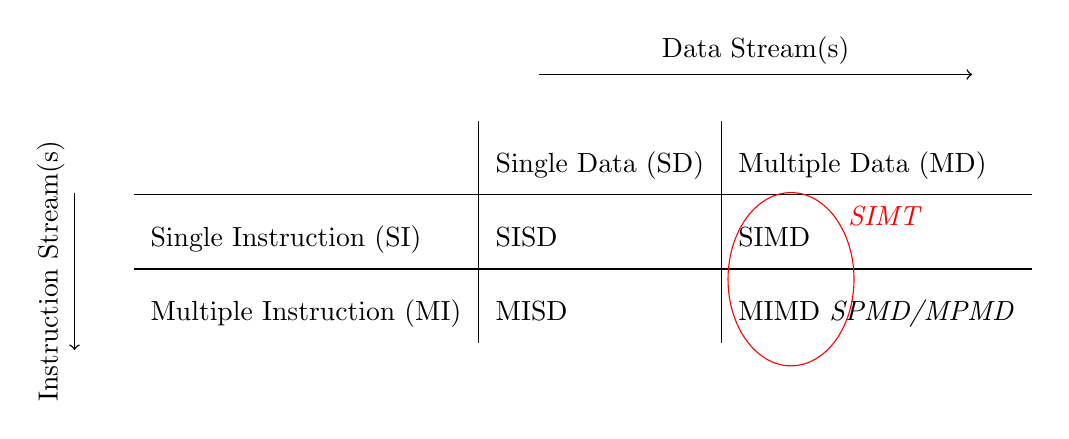
\begin{tikzpicture}
\node (table) {\arraycolsep=1.4pt\def\arraystretch{2.2}
\begin{tabular}{l | l | l}
 & Single Data (SD) & Multiple Data (MD) \\
 \hline 
Single Instruction (SI) & SISD & SIMD \\
\hline 
Multiple Instruction (MI) & MISD & MIMD \textit{SPMD/MPMD} \\
\end{tabular}
};
\draw [->,line width=.5pt] (-0.5,2) -- (5,2) node[midway, above] {Data Stream(s)};
\draw [->,line width=.5pt] (-6.4,0.5) -- (-6.4,-1.5) node[rotate=180,sloped, midway, above] {Instruction Stream(s)};
\draw [red] (2.7,-.6) ellipse (.8cm and 1.1cm) node[xshift=1.2cm,yshift=.8cm] {\textit{SIMT}};
%\draw[decoration={brace,raise=5pt},line width=1pt,decorate]
%  (5,0.4) -- node[right=6pt,yshift=5pt] {\textit{SIMT}} (5,-1.5);
\end{tikzpicture}
\caption{Flynn taxonomy for execution models completed with SPMD and SIMT models}
\label{tab:1_HPC:taxonomy_flynn}
\end{table}

\begin{figure}
\resizebox {.24\columnwidth} {!} {
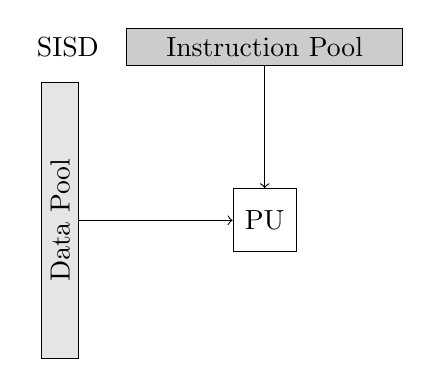
\begin{tikzpicture}
\draw (0.1,5.2) node {SISD}; 
\node (rect) at (2.6,5.2) [draw,minimum width=3.5cm,fill=black!20] (ip) {Instruction Pool};
\node (rect) at (0,3) [rotate=90,draw,minimum width=3.5cm,fill=black!10] (dp) {Data Pool};
\node (rect) at (2.6,3) [draw,minimum width=.8cm,minimum height=.8cm] (pu1) {PU};
\draw [->] (ip) -- (pu1);
\draw [->] (dp) -- (pu1);
\end{tikzpicture}
}
\resizebox {.24\columnwidth} {!} {
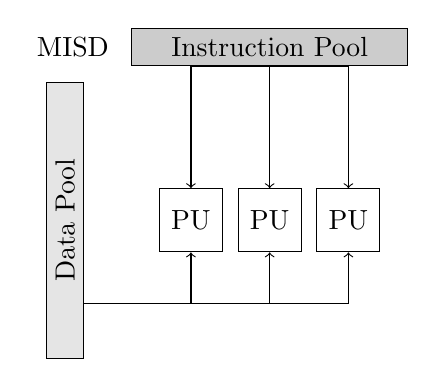
\begin{tikzpicture}
\draw (0.1,5.2) node {MISD}; 
\node (rect) at (2.6,5.2) [draw,minimum width=3.5cm,fill=black!20] (ip) {Instruction Pool};
\node (rect) at (0,3) [rotate=90,draw,minimum width=3.5cm,fill=black!10] (dp) {Data Pool};
\node (rect) at (1.6,3) [draw,minimum width=.8cm,minimum height=.8cm] (pu1) {PU};
\node (rect) at (3.6,3) [draw,minimum width=.8cm,minimum height=.8cm] (pu2) {PU};
\node (rect) at (2.6,3) [draw,minimum width=.8cm,minimum height=.8cm] (pu3) {PU};

\draw[<-] (pu1.north) |-  (ip.south); 
\draw[<-] (pu2.north) |-  (ip.south);
\draw[<-] (pu3.north) |-  (ip.south);

\draw[<-]  (pu1.south) |- ([yshift=-30pt]dp.south);
\draw[<-]  (pu2.south) |- ([yshift=-30pt]dp.south);
\draw[<-]  (pu3.south) |- ([yshift=-30pt]dp.south);

\end{tikzpicture}
}
\resizebox {.24\columnwidth} {!} {
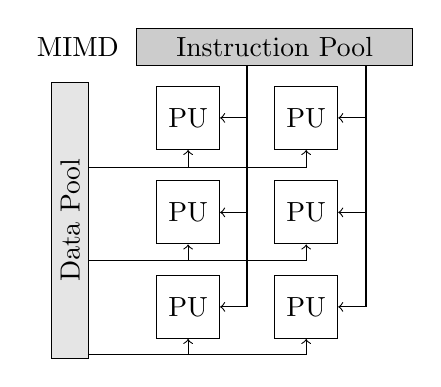
\begin{tikzpicture}
\draw (0.1,5.2) node {MIMD}; 
\node (rect) at (2.6,5.2) [draw,minimum width=3.5cm,fill=black!20] (ip) {Instruction Pool};
\node (rect) at (0,3) [rotate=90,draw,minimum width=3.5cm,fill=black!10] (dp) {Data Pool};
\node (rect) at (1.5,4.3) [draw,minimum width=.8cm,minimum height=.8cm] (pu1) {PU};
\node (rect) at (1.5,3.1) [draw,minimum width=.8cm,minimum height=.8cm] (pu2) {PU};
\node (rect) at (1.5,1.9) [draw,minimum width=.8cm,minimum height=.8cm] (pu3) {PU};
\node (rect) at (3,4.3) [draw,minimum width=.8cm,minimum height=.8cm] (pu4) {PU};
\node (rect) at (3,3.1) [draw,minimum width=.8cm,minimum height=.8cm] (pu5) {PU};
\node (rect) at (3,1.9) [draw,minimum width=.8cm,minimum height=.8cm] (pu6) {PU};

\draw[<-]  (pu1.south) |- ([yshift=19pt]dp.south);
\draw[<-]  (pu4.south) |- ([yshift=19pt]dp.south);

\draw[<-]  (pu2.south) |- ([yshift=-14.5pt]dp.south);
\draw[<-]  (pu5.south) |- ([yshift=-14.5pt]dp.south);

\draw[<-]  (pu3.south) |- ([yshift=-48.5pt]dp.south);
\draw[<-]  (pu6.south) |- ([yshift=-48.5pt]dp.south);

\draw[->] ([xshift=-10pt]ip.south) |- (pu1.east);
\draw[->] ([xshift=-10pt]ip.south) |- (pu2.east);
\draw[->] ([xshift=-10pt]ip.south) |- (pu3.east);

\draw[->] ([xshift=33pt]ip.south) |- (pu4.east);
\draw[->] ([xshift=33pt]ip.south) |- (pu5.east);
\draw[->] ([xshift=33pt]ip.south) |- (pu6.east);

%\draw[<-]  (pu2.south) |- ([yshift=-30pt]dp.south);
%\draw[<-]  (pu3.south) |- ([yshift=-30pt]dp.south);

%\draw [->] (ip) -- (pu1);
%\draw [->] (dp) -- (pu1);
\end{tikzpicture}
}
\resizebox {.24\columnwidth} {!} {
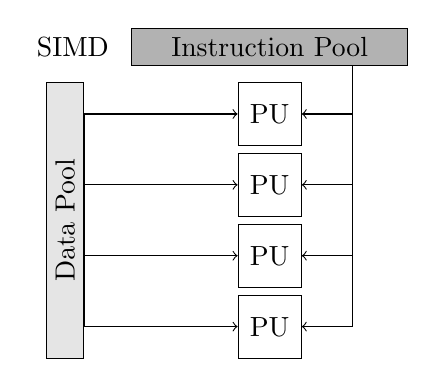
\begin{tikzpicture}
\draw (0.1,5.2) node {SIMD}; 
\node (rect) at (2.6,5.2) [draw,minimum width=3.5cm,fill=black!30] (ip) {Instruction Pool};
\node (rect) at (0,3) [rotate=90,draw,minimum width=3.5cm,fill=black!10] (dp) {Data Pool};
\node (rect) at (2.6,4.35) [draw,minimum width=.8cm,minimum height=.8cm] (pu1) {PU};
\node (rect) at (2.6,3.45) [draw,minimum width=.8cm,minimum height=.8cm] (pu2) {PU};
\node (rect) at (2.6,2.55) [draw,minimum width=.8cm,minimum height=.8cm] (pu3) {PU};
\node (rect) at (2.6,1.65) [draw,minimum width=.8cm,minimum height=.8cm] (pu4) {PU};
%\draw [->] ([yshift=2.35cm]dp) -- (pu1);
\draw[->] (dp.south) |- (pu1.west);
\draw[->] (dp.south) |- (pu2.west);
\draw[->] (dp.south) |- (pu3.west);
\draw[->] (dp.south) |- (pu4.west);

\draw[->] ([xshift=30pt]ip.south) |- (pu4.east);
\draw[->] ([xshift=30pt]ip.south) |- (pu3.east);
\draw[->] ([xshift=30pt]ip.south) |- (pu2.east);
\draw[->] ([xshift=30pt]ip.south) |- (pu1.east);
%\draw[arrow] (Small2B.north)--(Small2B|-Big2.south);s
%\draw [->] (dp) -- (pu1);
\end{tikzpicture}
}
\caption{Flynn taxonomy schematic representation of execution models}
\label{fig:1_HPC:flynn_taxonomy}
\end{figure}

In this classification~\cite{flynn1972some} from 1972, Michael J. Flynn presents the SISD, MISD, MIMD, and SIMD models.
Each of those execution models, presented on table~\ref{tab:1_HPC:taxonomy_flynn} and figure~\ref{fig:1_HPC:flynn_taxonomy}, corresponds to a specific machine and function.

\subsection{Single Instruction, Single Data: SISD}
This is the model corresponding to a single core CPU like in the Von Neumann model. 
This sequential model takes one instruction, operates on one data and the result is then stored and the process continues over. 
SISD is important to consider for a reference computational time and will be taken into account in the next part for Amdahl's and Gustafson's laws.

\subsection{Multiple Instructions, Single Data: MISD}
This model can correspond to a pipelined computer.
Different operations flows are applied to the datum, which is transfered to the next computational unit and so on. 
This is the least common execution model.


\subsection{Multiple Instructions, Multiple Data: MIMD}
In MIMD every element executes its own instructions flow on its own data set. 
This can represent the behavior of a processor using several cores, threads or even the different nodes of a supercomputer cluster. 
Two subcategories are identified in this model: SPMD and MPMD.

\subsubsection{SPMD}
The Single Program Multiple Data model, SPMD, is the most famous parallelism way for HPC purpose: each process executes the same program. 
The programs are the same but does not share the same instruction counter. 
This model was proposed for the first time in \cite{darema1988single} in 1988 using Fortran.
This is the common approach working with runtime like MPI. 
The programs are the same and the executions are independent but based on their ID the processes will target different data. 

\subsubsection{MPMD}
The Multiple Program Multiple Data model is also know for HPC: Some of the processes may execute programs for different purposes.  
Generally with a separation between a main program generating data for sub-programs. 
This is the model on which we work in part II, regarding the Langford problem resolution using a master program generating tasks for the slaves CPUs/GPGPUs programs.

\subsection{Single Instruction, Multiple Data: SIMD}
This execution model corresponds to many-core architectures like a GPU. 
SIMD can be extended from 2 to 16 elements for classical CPUs to hundreds and even thousands of core for GPGPUs. 
In the same clock cycle, the same operation is executed on every process on different data. 
A good example is the work on matrices with stencils: same instruction executed on every element of the matrix in a synchronous way: the processing elements share one instruction unit and program counter. 

\subsection{SIMT}
\index{Single Instruction Multiple Threads}
We find another characterization to describe the new GPUs architecture: Single Instruction, Multiple Threads. 
This first appears in one of NVIDIA's company paper~\cite{lindholm2008nvidia}. 
This model describes a combination of MIMD and SIMD architectures, every block of threads is working with the same control processor on different data and in such a way that every block has its own instruction counter.  
This is the model we describe in part~\ref{sec:CUDA}, used for the \textit{warps} model in NVIDIA CUDA.

\section{Memory}
\label{sec:NORMA}
In addition to the execution model and parallelism, the memory access patterns have a main role in performances in SIMD and MIMD. 
In this classification we identify three categories: UMA, NUMA and NoRMA for shared and distributed cases. 
This classification has been pointed out in the Johnson's taxonomy\cite{johnson1988completing}.

%We can also find Error-Correcting Code, ECC, memory which implements a bunch of data correction algorithm to guaranty the validity of them when error is not allowed. 

%\todo{MCDRAM}
%\todo{3D memory}

\begin{figure}
\centering 
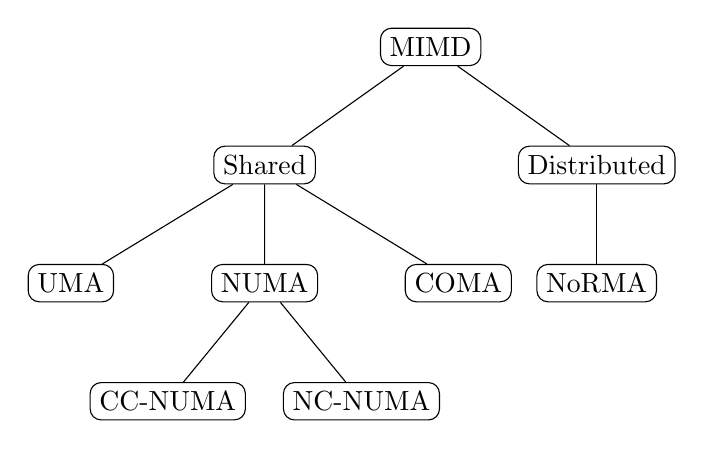
\begin{tikzpicture}[
   every node/.style = {
   level distance=1em,
   shape=rectangle, 
   rounded corners,
   draw, 
   align=center,
    top color=white%, 
   % bottom color=blue!20
   }]]
   \node {MIMD} [sibling distance=12em]
   child { node {Shared} [sibling distance=7em]
   child{node {UMA}} 
   child{node {NUMA}
   child{node {CC-NUMA}}
   child{node {NC-NUMA}}
   }
   child{node {COMA}}
   }
   child { node {Distributed}
   child { node {NoRMA}}
   };
\end{tikzpicture}
\caption{MIMD memory models}
\label{fig:1_HPC:mimd_memory_model}
\end{figure}

Those different types of memory for SIMD/MIMD model are summarized in figure~\ref{fig:1_HPC:mimd_memory_model}, and presented below.

\subsection{Shared memory}
%In case of the SISD the memory access is just serial and no really rules needs to be set for its usage. 
Several kinds of memory models are possible when it comes to multi-threaded and multi-cores execution models like MIMD or SIMD models.
We give a description of the most common shared memories architectures. 

\hspace*{-2cm}
\begin{figure}
\centering 
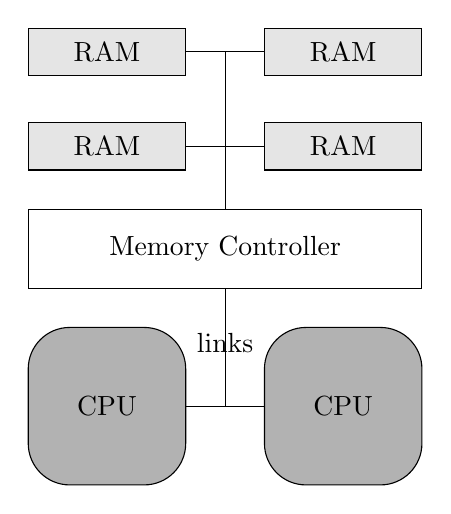
\begin{tikzpicture}
   \draw [rounded corners=15pt,fill=black!30] (0,0) rectangle (2,2) node[pos=.5] {CPU};
   \draw [rounded corners=15pt,fill=black!30] (3,0) rectangle (5,2) node[pos=.5] {CPU};

   \draw (0,2.5) rectangle (5,3.5) node[pos=.5] {Memory Controller};

   \draw (0,4) [fill=black!10] rectangle (2,4.6) node[pos=.5] {RAM};
   \draw (0,5.2) [fill=black!10] rectangle (2,5.8) node[pos=.5] {RAM};

   \draw (3,4) [fill=black!10] rectangle (5,4.6) node[pos=.5] {RAM};
   \draw (3,5.2) [fill=black!10] rectangle (5,5.8) node[pos=.5] {RAM};

   \draw [-] (2,1) -- (3,1);
   \draw [-] (2.5,1) -- (2.5,2.5);
	%\node at (2.5,2.2) {SDR, DDR, QDR};
	\node at (2.5,1.8) {links};

	\draw [-] (2.5,3.5) -- (2.5,5.5);
	\draw [-] (2,4.3) -- (3,4.3);
	\draw [-] (2,5.5) -- (3,5.5);
\end{tikzpicture}
\hspace{2cm}
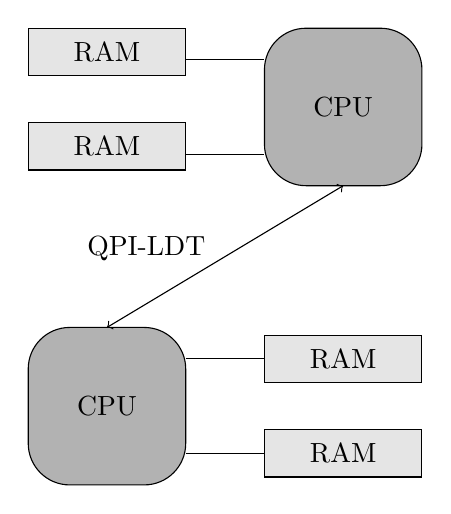
\begin{tikzpicture}
	\draw [rounded corners=15pt,fill=black!30] (0,0) rectangle (2,2) node[pos=.5] {CPU};
	\draw (3,0.1) [fill=black!10] rectangle (5,0.7) node[pos=.5] {RAM};
	\draw (3,1.3) [fill=black!10] rectangle (5,1.9) node[pos=.5] {RAM};
	\draw [-] (2,0.4) -- (3,0.4);
	\draw [-] (2,1.6) -- (3,1.6);

	\draw [rounded corners=15pt,fill=black!30] (3,3.8) rectangle (5,5.8) node[pos=.5] {CPU};
	\draw (0,4) [fill=black!10] rectangle (2,4.6) node[pos=.5] {RAM};
	\draw (0,5.2) [fill=black!10] rectangle (2,5.8) node[pos=.5] {RAM};
	\draw [-] (2,4.2) -- (3,4.2);
	\draw [-] (2,5.4) -- (3,5.4);

	\draw [<->] (1,2) -- (4,3.8);
	\node at (1.5,3) {QPI-LDT};
\end{tikzpicture}
%\hspace{1cm}
%\begin{tikzpicture}
%	\draw [rounded corners=15pt] (1,0) rectangle (3,2) node[pos=.5] {CPU};
%	\draw [rounded corners=15pt] (1,3.8) rectangle (3,5.8) node[pos=.5] {CPU};
%
%	\draw (0,2.1) rectangle (2,2.8) node[pos=.5] {RAM};
%	\draw (0,3.2) rectangle (2,3.8) node[pos=.5] {RAM};
%	
%	\draw (3,2.2) rectangle (5,2.8) node[pos=.5] {RAM};
%	\draw (3,2.2) rectangle (5,3.8) node[pos=.5] {RAM};
%
%\end{tikzpicture}
\caption{UMA vs NUMA memory models}
\label{fig:1_HPC:UMA_NUMA}
\end{figure}

\subsubsection{UMA}
\index{Unified Memory Access}
The Uniform Memory Access architecture have a global memory shared by every threads or cores. 
In UMA every processor uses its own cache as local private memory and the accesses consume the same amount of time: the addresses can be accessed directly by each processor which makes the access time ideal. 
The downside is that more processors require more buses and thus UMA is hardly scalable. 
The cache consistency problem also appears in this context and will be discussed in next part: indeed, if a data is loaded in one processor cache and modified, this information has to be spread to the memory and maybe other processes cache. 

With the arising of accelerators like GPUs and their own memory, some constructors found ways to create UMA with heterogeneous memory: AMD created the heterogeneous UMA, hUMA~\cite{rogers2013amd} in 2013, allowing CPU and GPU to target the same memory area, but the performances still need to be checked in an HPC context.

\subsubsection{NUMA}
\index{Non Uniform Memory Access}
In Non Uniform Memory Access every processor has access to its own private memory but allows other processors to access it though Lightning Data Transport, LDT, or Quick Path Interconnect, QPI, for Intel architectures. 

As mentioned for the UMA memory, even if the processors do not directly access to the memory cache, coherency is important. 
Two methods are possible: on one hand, the most used is Cache-Coherent NUMA (CC-NUMA) where protocols are used to keep data coherency through the memory. 
On the other hand No Cache NUMA (NC-NUMA) forces the processes to avoid cache utilization and write results to main memory, losing all the benefits of caching data. 

\subsubsection{COMA}
\index{Cache-Only Memory Access}
In Cache-Only Memory Accesses, the whole memory is see as a cache shared by all the processes processes.
An \textit{Attraction memory} pattern is used to \textit{attract} the data near the process that will use them. 
This model is less commonly use and, in best cases, lead to same results as NUMA.

\subsection{Distributed memory}
\index{No Remote Memory Access}
The previous models are dedicated on shared memory, if the processes can access memory of their neighbors processes. 
In some cases, like supercomputers, it would be too heavy for processors to handle the requests of all the others through the network. 
Each process or node will then possess its own local memory, that can be shared only between local processes. 
Then, in order to access to other nodes memory, communications through the network have to be done and copied into local memory. 
This distributed memory model is called No Remote Memory Access (NoRMA).
This requires transfer schemes, that have to be added to local read-write accesses.

\section{Performances characterization in HPC}
In the previous parts we described the different execution models and memory models for HPC. 
Based on those aspects we need to be able to emphasis the performances of a computer and a cluster. 

The performance can be of several kinds. 
It can first be defined by the speed of the processors themselves with the frequency defined in GHz. 
We define the notion of \textit{cycle} to be the number that determine the speed of a processor. 
This is the amount of time between two pulses of the oscillator at the best frequency. 
Higher cycles per seconds is better. 
It can be used to estimate the highest computational power of a machine. 
This information is not perfect because the ALU is not busy all the time due to memory accesses, communications or side effects. 
Then we have to go through more accurate ways to characterize performance.

\subsection{FLOPS}

\index{Floating-point Operations Per Second}

The FLoating point Operations Per Second value considers the number of floating-point operation that the system will execute in a second. 
Higher FLOPS is better and this is the most common scale used to consider supercomputers computational power. 
For a cluster we can compute the theoretical FLOPS (peak) based on the processor frequency in GHz with:
\begin{equation}
FLOPS_{cluster} = \#nodes \times \frac{\#sockets}{\#node} \times \frac{\#cores}{\#socket} \times \frac{\#GHz}{\#core} \times \frac{FLOPS}{cycle}
\end{equation}
With $\#nodes$ the number of computational node of the system, $\frac{\#sockets}{\#node}$ the number of sockets (=processors) per node, $\frac{\#cores}{\#socket}$ the number of cores in the processor, $\frac{\#GHz}{\#core}$ the frequency of each core and finally $\frac{\#FLOP}{\#cycle}$ the number of floating-point operations per cycles for this architecture. 


Table~\ref{tab:1_HPC:flops_year} presents the scale of FLOPS and the year of the first world machine reached this step.
The next milestone, the exascale, is expected to be reach near 2020.  

\begin{table}
\[\arraycolsep=1.4pt\def\arraystretch{2.2}
\begin{tabular}{| l | l | l || l | l | l |}
\hline
	%\rowstyle{\bfseries}
	\textbf{Name} & \textbf{FLOPS} & \textbf{Year} & \textbf{Name} & \textbf{FLOPS} & \textbf{Year} \\
	\hline
	\hline
	kiloFLOPS & $10^{3}$ & & petaFLOPS  & $10^{15}$ & 2005 \\ 
	\hline
	megaFLOPS & $10^{6}$ & & exaFLOPS   & $10^{18}$ & 2020 ? \\
	\hline
	gigaFLOPS & $10^{9}$ & $\approx$ 1980  & zettaFLOPS & $10^{21}$ & \\
	\hline
	teraFLOPS & $10^{12}$ & 1996 & yottaFLOPS & $10^{24}$ & \\
	\hline
	\end{tabular}
	\]
	\caption{Floating-point Operation per Second and years of reach in HPC.}
	\label{tab:1_HPC:flops_year}
\end{table}

Even though, many ways exist to measure computer's performance: Instructions Per Seconds (IPS), Instructions per Cycle (IPC) or Operations Per Seconds (OPS) but none of these consider what an instruction or operation is. 
Thus, floating point can be considered as a basis, and a comparison can be provided. 


\subsection{Power consumption}
Another way to consider machine performance is to estimate the number of operations regarding the power consumption. 
It considers all the previous metrics like FLOPS, IPS, IPC or OPS. 
Benchmarks like the Green500 consider the FLOPS delivered over the watts consumed. 
For nowadays architectures the many-cores accelerated architectures with GPUs seems to deliver the best FLOPS per watt ratio.

\subsection{Scalability}

After considering architectures evaluation, one have to measure the applications performances.
The scalability expresses the way a program reacts to parallelism. 
When an algorithm is implemented on a serial machine and is ideal to solve a problem, one may consider to use it on more than one core, socket, node or even cluster. 
Indeed, while using more resources one may expect less computation time or access larger instances, or a combination of both. 
This is completely dependent of the algorithm's parallelization and is expressed through scalability. 
A scalable program will scale on as many processors as provided, whereas a poorly scalable one will give same of even worst results than the serial code.  
Scalability can be approached using speedup and efficiency.

\subsection{Speedup and efficiency}
The latency is the time required to complete a task in a program.
\index{Latency} 
Lower latency is better. 

The speedup compares the latency of both sequential and parallel algorithm. 
In order to get relevant results, one may consider the given best serial program against the best parallel implementation.

Considering $n$, the number of processes, and $n=1$ the sequential case.
$T_n$ is the execution time working on $n$ processes and $T_1$ the sequential execution time. 
The speedup can be defined using the latency by the formula: 
\index{Speedup}
\begin{equation}
\text{speedup} = S_n =  \frac{T_1}{T_n}
\end{equation}

\begin{figure}
\centering 
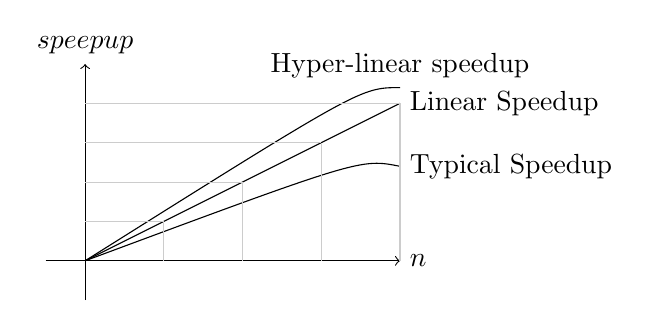
\begin{tikzpicture}
	\draw[->] (-.5,0) -- (4,0) node[right] {$n$};
	\draw[->] (0,-.5) -- (0,2.5) node[above] {$speepup$};
	\draw (0,0) -- (4,2) node[right] {\text{Linear Speedup}};
	\draw (0,0) .. controls (3.5,1.3) .. (4.,1.2) node[right] {\text{Typical Speedup}} ;
	\draw (0,0) .. controls (3.5,2.2) .. (4.,2.2) node[above] {\text{Hyper-linear speedup}} ;
   \draw[black!20] (1,0) -- (1,.5);
   \draw[black!20] (2,0) -- (2,1);
   \draw[black!20] (3,0) -- (3,1.5);
   \draw[black!20] (4,0) -- (4,2);
   \draw[black!20] (0,.5) -- (1,.5);
   \draw[black!20] (0,1) -- (2,1);
   \draw[black!20] (0,1.5) -- (3,1.5);
   \draw[black!20] (0,2) -- (4,2);
\end{tikzpicture}
\caption{Observed speedup: linear, typical and hyper-linear speedups}
\label{fig:1_HPC:speedup_obs}
\end{figure}


In addition to speedup, the efficiency is defined by the speedup divided by the number of workers: 
\index{Efficiency}
\begin{equation}
\text{efficiency} = E_n = \frac{S_n}{n} = \frac{T_1}{nT_n}
\end{equation}
The efficiency, usually expressed in percent, represents the evolution of the code stability to growing number of processors. 
As the number of processes grows, a scalable application will keep an efficiency near 100\%.


As shown on figure \ref{fig:1_HPC:speedup_obs} several kinds of speedup can be observed. 
\paragraph{Linear, reference speedup: }
The linear speedup usually represents the target for every program in HPC. 
Indeed, having a constant efficiency, which means that the speedup grows linearly as the number of processors grows is the ideal case. 
Codes fall typical into two cases, typical and hyper-linear speedup. 
\paragraph{Typical speedup: }
This represents the most common observed speedup. 
As the number of processors grows, the program faces several of the HPC walls like communications wall or memory wall. 
The increasing number of computational power may be lost in parallel overhead, and efficiency reduced. 
\paragraph{Hyper-linear speedup: }
In some cases we observe an hyper-linear speedup, meaning that the results in parallel are even better than the ideal case. 
This increasing efficiency can occur if the program fits exactly in memory for less data on each processor or even fit perfectly for the cache utilization. 
The parallel algorithm can also be more efficient than the sequential one, for example with optimizations application: if the search space is divided over processing units, one can find good solutions more quickly.

\subsection{Amdahl's and Gustafson's law}
The Amdahl's and Gustafson's laws are ways to evaluate the maximal possible speedup for an application taking into account different characteristics. 

\subsubsection{Amdahl's law}
\index{Amdahl's law}
The Amdahl's law\cite{amdahl1967validity} is used to find the theoretical speedup in latency of a program.
We can separate a program into two parts, the one that can be executed in parallel with optimal speedup and the one that is intrinsically sequential.
The law states that even if we reduce the parallel part using an infinity of processes the sequential part will reach 100\% of the total computation time. 

Extracted from the Amdahl paper the law can be written as: 

\begin{equation}
S_n = \frac{1}{Seq + \frac{Par}{n}}
\end{equation}

Where $Seq$ and $Par$ respectively the sequential and parallel ratio of a program $( Seq + Par = 1 )$.
Here if we use up to $n=\inf$ processes, $S_n \leq \frac{1}{Seq}$ the sequential part of the code become the most time consuming. 

And the efficiency become:
\begin{equation}
E_n = \frac{1}{n\times Seq + Par}
\end{equation}

\begin{figure}
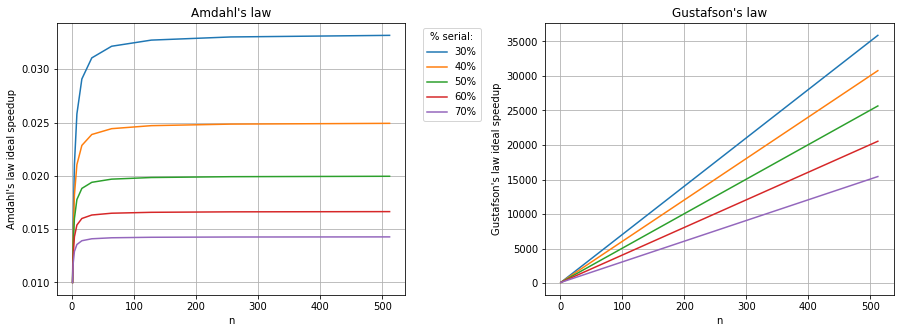
\includegraphics[width=\textwidth]{\locpath/figures/chap1/speedup_laws.png}
\caption{Theoretical speedup for Amdahl's (left) and Gustafson's (right) law}
\label{fig:1_HPC:speedup_laws}
\end{figure}

A representation of Amdahl's speedup is presented on Fig.~\ref{fig:1_HPC:speedup_laws} with varying percentage of serial part. 
%The parallel part is like $Par = (100-Ser)\%$.

\subsubsection{Gustafson's law}
\index{Gustafson's law}
The Amdahl's law focuses on time with problem of the same size. 
John L. Gustafson's idea is that using more computational units and the same amount of time, the problem size can grow accordingly. 
He considered a constant computation time with evolving problem, growing the size accordingly to the number of processes. 
Indeed the parallel part grows as the problem size does, reducing the percentage of the serial part for the overall resolution.

The speedup can now be estimated by:
\begin{equation}
S_n = Seq + Par \times n
\end{equation}

And the efficiency: 
\begin{equation}
E_n = \frac{Seq}{n} + Par
\end{equation}


Both Amdahl's and Gustafson's law are applicable and they represent two solutions to check the speedup of our applications. 
\textbf{The strong scaling}\index{Strong scaling}, looking at how the computation time vary evolving only the number of processes, not the problem size. 
\textbf{The weak scaling}\index{Weak scaling}, at the opposite to strong scaling, regards to how the computation time evolutes varying the problem size but keeping the same amount of work per processes. 

\section{Conclusions}

In this chapter we presented the different basic considerations to be able to understand HPC: the Von Neumann model that is implemented in every nowadays architecture; the Flynn taxonomy that is in constant evolution with new paradigms like recent SIMT from NVIDIA. 
We also presented the memory types that will be used at different layers in our clusters, from node memory, CPU-GPGPU shared memory space to global fast shared memory. 
We finished by presenting the most important laws with Amdahl's and Gustafson's laws.
We introduced the concept of strong and weak scaling that will lead our tests through all the examples in Part II and Part III.

Those models have now to be confronted to the reality with hardware implementation and market reality, the vendors. 
The next chapter introduces chronologically hardware enhancements and their optimization and always keeps a link with the models presented in this part.

As there is always a gap between models and implementation we will have to find ways to rank and characterize those architectures. 
This will be discussed in the last chapter. 
